\documentclass[../main.tex]{subfiles}
\graphicspath{{\subfix{../IMAGES/}}}

\begin{document}

\localtableofcontents
\subsection{Dessin technique}
Contient des vues de l'objet avec des dimensions, des exigences de précisions, avec un cadre formel...\\

\quad \underline{Langage normalisé :}\\
Unification des codes/formats de représentation/ unité de mesure... par ISO.\\

\quad \underline{Projection orthogonal :}\\
Plan de projection perpendiculaire à la direction de projection. Direction de projection perpendiculaire à 1 ou plusieurs faces de l'objet.\\

\quad \underline{Cube de projection :}\\
On place l'objet dans un cube (face du cube parallèle aux faces principales de l'objet). On déplie ensuite les faces pour faire apparaître les 6 faces sur un même plan.\\
\begin{minipage}{.5\textwidth}
    Méthode de projection : symbole sur le plan :
\end{minipage}
\hfill
\begin{minipage}{.5\textwidth}
    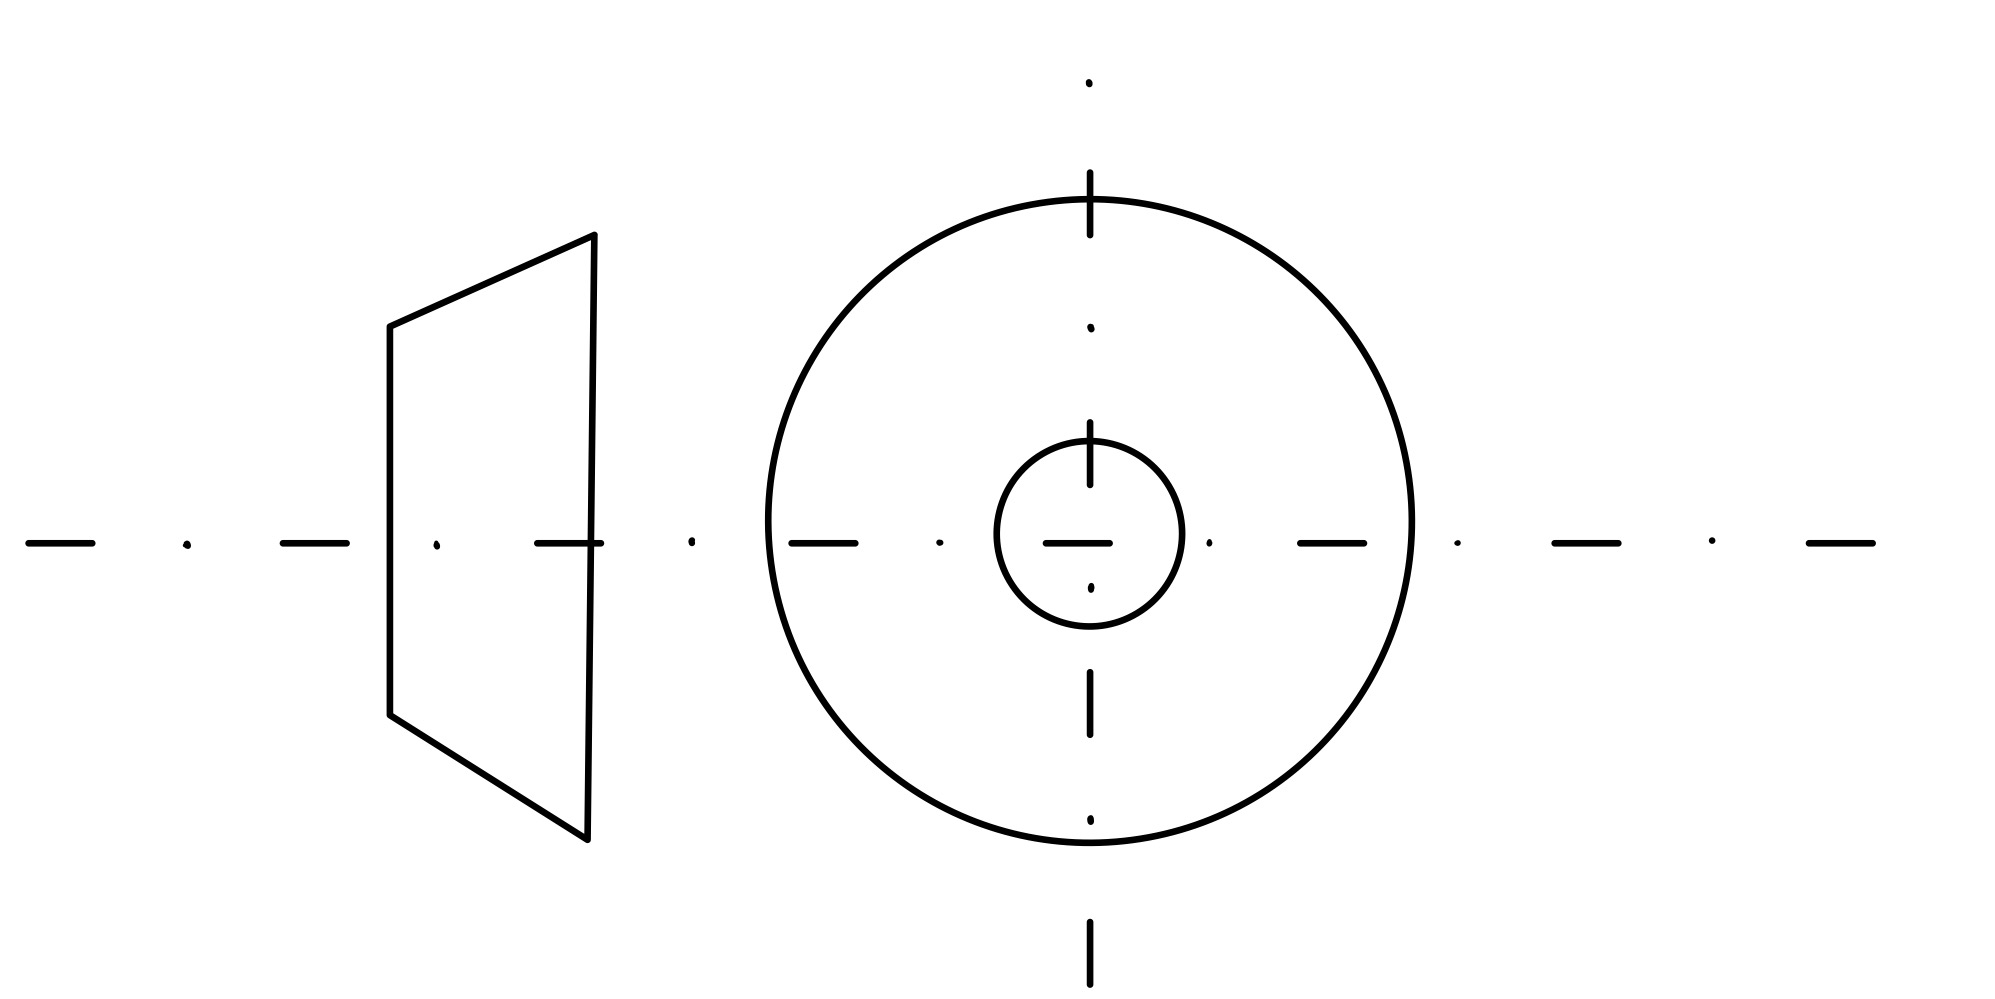
\includegraphics[width=\textwidth]{IMAGES/constru/symboleiso.jpeg}
\end{minipage}

\quad \underline{Choix des vues :}\\
Vue de face : celle qui a le plus d'infos;\\
Les deux autres : celles avec des arêtes visibles.\\
\color{gray} 2 vues suffisent pour une pièce avec un trou; une vue pour des pièces de révolution.\color{black}\\

\quad \underline{Correspondance des vues :}\\
Méthode de projection plus proportions respectées : alignement des vues et correspondance des dimensions.

\subsubsection{Types de vues}
\quad \underline{Partielle :}\\
Principe : 1 partie de la vue est coupé par trait ondulé\\

\quad \underline{Interrompue :}\\
Principe : raccourcir des objets long (couper par deux ondulations)\\

\quad \underline{$\frac{1}{2}$ vue et $\frac{1}{4}$ vue :}\\
Principe : Si pièce possède des symétries planaires, on peut les représenter en demie ou quart de vue avec des trait parallèles pour symétrie.\\

\quad \underline{Détail :}\\
Principe : Vue secondaire, représentation en échelle agrandie.\\

\quad \underline{Auxiliaire :}\\
Principe : Placement libre de la vue, représentée par une lettre et une flèche.\\

\begin{figure}[hbt!]
    \centering
    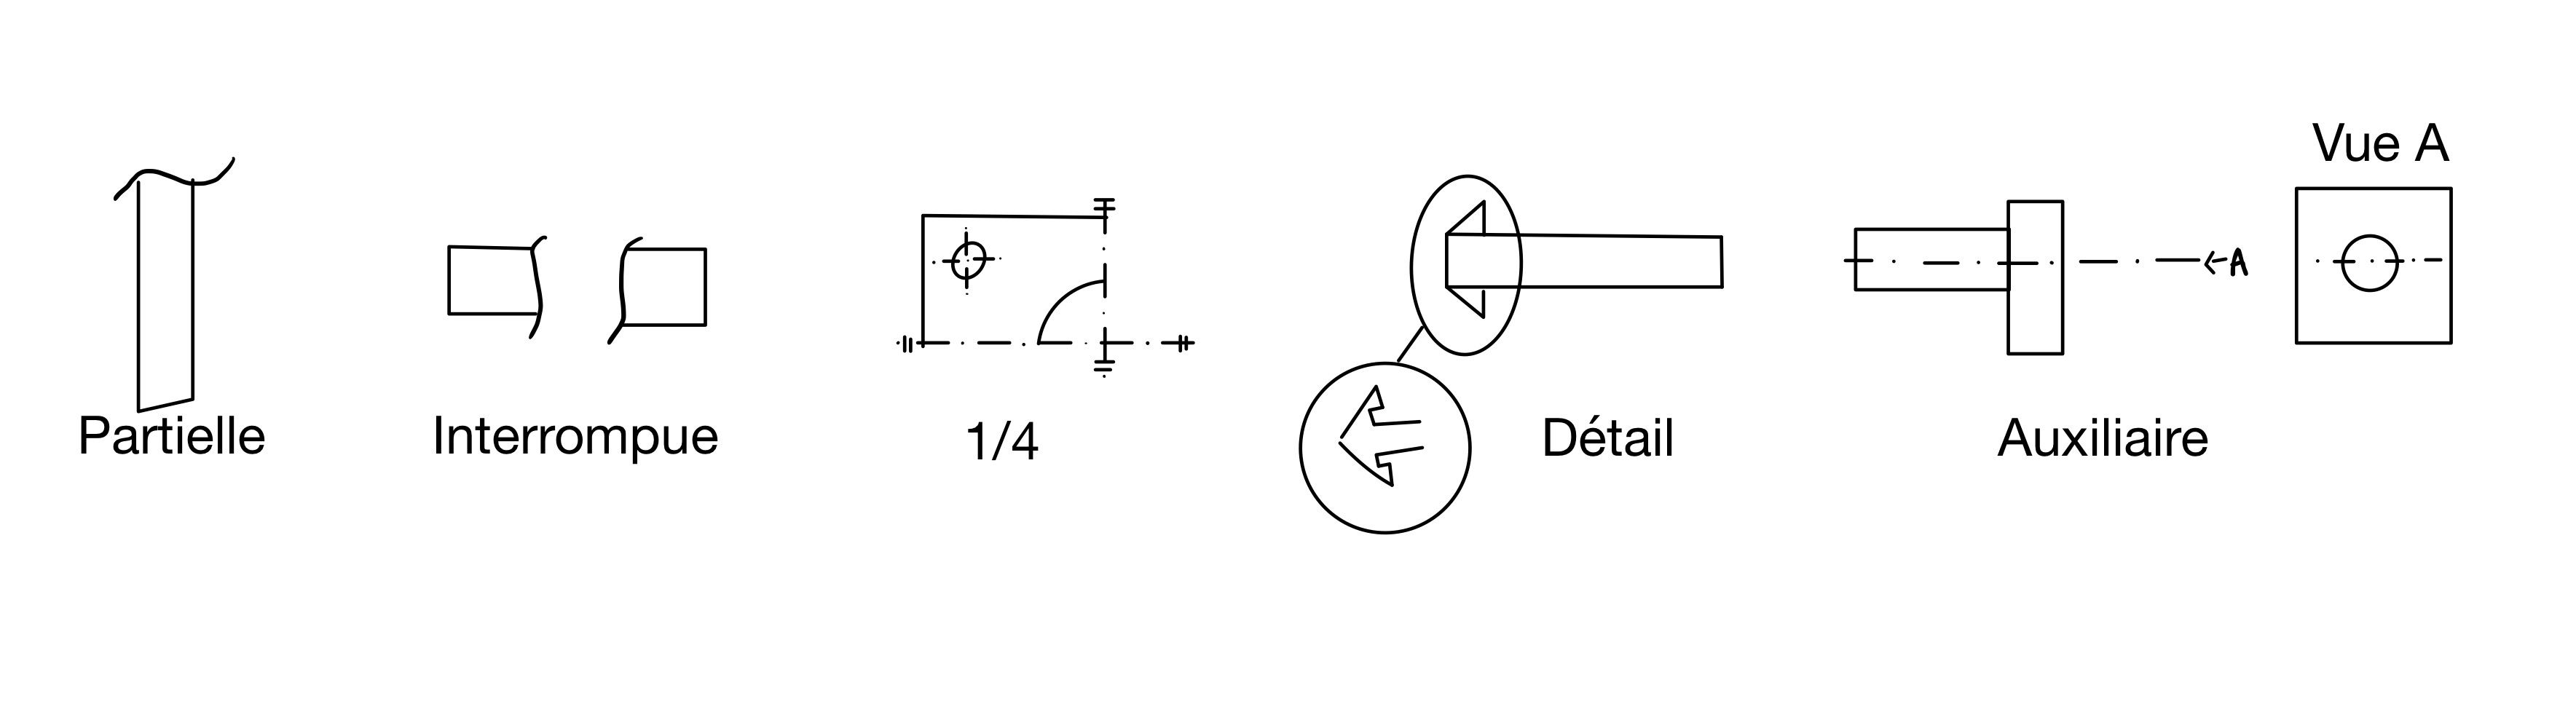
\includegraphics[width=\textwidth]{IMAGES/constru/vues.jpeg}
    \caption{Différents types de vues}
    
\end{figure}


\subsubsection{Projections axonométriques}
Limite projection orthogonale : pas d'information de profondeur avec une seule vue, si plusieurs vues, l'information est dissociée.\\
\underline{Principe :} Plan de projection perpendiculaire à la direction de projection. Direction de projection quelconque par rapport à la pièce. \\
\underline{Avantages :} Visuel intuitif de l'objet\\
\underline{Inconvénients :} Dimensions et angles non respectés.\\
Sans points de fuites. 
\begin{itemize}
    \item[$\bullet$] Perspective cavalière : vue depuis un point haut, face avant : vraie taille, latérale : .5 sur profondeur\\
    \item[$\bullet$] Perspective isométrique : 3 faces visible en 1 vue (3 angles égaux), direction de projection selon le vecteur (1,1,1), taille arrête : $\sqrt{\frac{2}{3}}\cdot$taille réelle\\
    \item[$\bullet$]Perspective dimétrique : 2 angles égaux\\
    \item[$\bullet$]Perspective trimétrique : direction de projection quelconque.\\
\end{itemize}

\subsubsection{Coupes et sections}
Trait mixte fin puis fort aux extrémités. Direction observation perpendiculaire au plan de coupe. Sens observation : double flèche. Trait interrompus interdit. 

\quad \underline{Cas des nervures :}\\
Une nervure est un élément de renforcement d'une pièce mécanique pour limiter les contraintes et optimiser la rigidité de la pièce. Elle n'est pas hachurée pour ne pas surcharger le dessin.\\

\quad \underline{Demi-coupe :}\\
Seule la moitié est représentée en coupe et l'autre moitié en vue extérieure.\\

\quad \underline{Coupe brisée :}\\
On coupe la pièce suivant un axe non linéaire.\\

\quad \underline{Coupes locales/partielles :}\\
Coupe ne couvre pas toute la pièce mais seulement une zone.\\

\quad \underline{Section :}\\
Seul le volume coupé est représenté (pas ce qu'il y a derrière).\\

\quad \underline{Section rabattue :}\\
La section est insérée dans la vue principale.\\


\subsection{Normalisation}
Processus de normalisation ISO : 
\begin{enumerate}
    \item Création d'une nouvelle norme\\
    \item Examen périodique ($\sim$ tous les 5ans)\\
    \item Révision de la norme?\\
\end{enumerate}
\textbf{Nom : ISO (N$^{\circ}$ norme) (année de révision)}\\
Arborescence : ISO (organisation supranationale) $\rightarrow$ standards, CEN, JISC (organisation internationale)$\rightarrow$ BSV, DIN, AFNOR, SNC... (organisation nationale)\\

\underline{Formats de papiers :} $A_0 = 1m^2$, rapport des côtés : $\sqrt{2}$, rapport des surfaces : 2. \textbf{Toujours en paysage! Sauf pour les A4}.\\

\quad \underline{Éléments graphiques permanents :}\\
Coordonnées, \textbf{Cartouche :} coin inférieur droit; désignation et n$^{\circ}$ pièce; échelle principale; masse et matière de la pièce; nom et date du dessinateur; formats, n$^{\circ}$et nombre de feuille.\\

\quad \underline{Échelle de représentations :}\\
Ratio de représentation sur la feuille par rapport à l'objet (X:1 agrandissement, 1:X réduction)

\subsubsection{Cotations}
Cylindrique : $\phi$, sphérique : $S\phi$, arc circulaire (arrondis, congés d'arètes) : R, arc circulaire : SRSurplat écartement : S ou SW, surplat carré : un carré, longueur arc : un pont.

\subsection{Principe de l'usinage}
Deux types : tournage ou fraisage. \\

\quad \underline{Formation de copeau :}\\
Arrachage de matière avec mouvement relatif matière/outil.\\

\quad \underline{Physique des matériaux :}\\
Forte contrainte local; grande déformation plastique; échauffement local élevé.\\

\quad \underline{Propriétés requises :}\\
Grande résistance à l'abrasion; grande limite élastique; grande dureté de surface.\\

\quad \underline{Matière outil de découpe :}\\
Carbure métalliques (cermet) :\\
Dureté et résistance à l'abrasion grande à haute température; très répandue, obtenu par frittage de poudre.\\
Aciers rapides supérieurs :\\
aciers alliés trempés (disque diamant); grande résistance mécanique; très bonne tenue à haute température. \\

\quad \underline{Liquide de coupe :}\\
Réduisent les frottements, limite dégagement de chaleur, réduit contraintes mécaniques et augmentent rendement énergétique. Il existe huile de coupe et solutions aqueuses. \\

\quad \underline{Choix des paramètres de coupe :}\\
Principe: choix de la vitesse de coupe telle que la température, l'effort de machine d'usinage et la puissance nécessaire à la coupe soient optimaux. \\
On peut faire varier, vitesse coupe : $V_c = d\pi N$, vitesse d'avance : $V_f = N f_z Z$ et profondeur de passe : $a_p$. \color{gray} Avec N : vitesse de rotation, Z: nombre de dents. Vitesse de coupe 4fois plus rapide avec cermet en moyenne.\color{black}\\


\quad \underline{Topologie pièce finie :}\\
Tournage avec mandrin : surfaces axi-symétriques\\
Fraisage avec étau de serrage : surfaces planes\\
Opération les plus courantes : chariotage(réduire épaisseur), dressage, alésage(trou), fraisage.\\

\quad \underline{Perçage :}\\
Avec un forêt, si borgne : fond de trou à 120$^{\circ}$, peut être fait avec tour/fraiseuse.\\

\quad \underline{Contraintes:}\\
 Arêtes rentrantes : toujours congés d'arêtes; sortantes : chanfreins à 45$^{\circ}$ sur toutes les arêtes vives.\\

\quad \underline{Qualité :}\\
Tournage : surface dressées/chariotées : stries concentriques; fraisage en bout/roulant : stries circulaire. \\

\subsection{État de surface}
Mesure topographique des défauts de surfaces réels. C'est une moyenne du profil. \\
Classe de rugosité : N suivi d'un nombre entre 1 et 12. \\
Ra : écart arithmétique : somme des surfaces au dessus de ligne moyenne / longueur de base.\\
De base : un V; si valeur exigée : $\sqrt{Ra 1.6}$; si obtenu par enlèvement de matière : $\overline{V}$; si obtenu sans enlèvement de matière : $V^{\circ}$.\\

\subsection{Tolérances dimensionnel}
Contrôle des côtes linéaires : réglette, micromètre, pied à coulisse...; côtes angulaires : rapporteur d'angle. \\
Tolérances : lim sup-lim inf\\
Système de tolérance : 1lettre + 1nombre : minuscule si dimension extérieure; majuscule si dimension intérieure. Nombre entre 1 (plus précis) et 18 (moins précis).\\

\quad \underline{Jeu :}\\
Jeu si J>0, serrage sinon.\\
$J_{min} = D_{min} - d_{max}$, $J_{max} = D_{max}-d_{min}$
Si $J_{min} > 0$ : jeu si $J_{max} < 0$: serrage, si les deux : incertain.\\
En général : classe arbre = classe alésage-1.\\

\subsection{Assemblage boulonnés}
Vissage : principal moyen d'assemblage ($\sim 70\%$). Maintient par adhérence, vis sollicitée en traction et pièce en compression. Plusieurs solutions de boulonnage :\\
\begin{enumerate}
    \item Vis et taraudage : le plus courant\\
    \item Vis et écrou : si taraudage impossible\\
    \item Goujon et écrou : si utilisation de vis impossible\\
\end{enumerate}


\quad \underline{Rôle du filetage :}\\
Liaison mécanique par obstacle. Le pas est la distance entre 2 filets successifs. Filetage normalisée :\\
1 seul filet; pas à droite par défaut; standards ISO : M pour métrique (G en pouces pour tuyauterie).\\

\quad \underline{Vis normalisées principales :}\\
Vis à tête cylindrique, 6 pans creux : avec clé Allen\\
Vis à tête hexagonale : serrage à clé à fourche\\
Tête conique, 6 pans creux : embase conique pour serrage\\

\quad \underline{Écrous normalisés principaux :}\\
Hex, auto-freiné avec anneau en polyamide. \\

\quad \underline{Clé de serrage :}\\
6 pans creux : Allen, inbus : serrage axial/axial\\
Hexagonale : clé à fourche (serrage radial), clé à pipe (serrage radial/axial).\\

\quad \underline{Rondelles normalisées principales :}\\
Rondelle plate : recommandé sur aluminium, prévient le tassement par matage\\
Rondelle grower : prévient contre desserrage (indentation de la pièce)\\

\quad \underline{Fabrication filetage intérieur :}\\
Avec un taraud : perçage de diamètre $D_B$ profond (avant-trou) puis taraudage. Avant-trou conique à 120$^{\circ}$. Taraudage jusqu'à : $\sim D_B$.\\

\quad \underline{Filetage métrique :}\\
Angle de filet : 60$^{\circ}$ avec diamètre avant-trou : $D_B = P-d$.\\
Si pas normal : $M\cdot d$, si pas fin : $M\cdot d\cdot P$\\
Contrainte de traction maximale donnée par $A_s$

\quad \underline{Filetage gaz :}\\
Étanche : filetage extérieur conique : $R\cdot d$ si extérieur et $Rp\cdot d$ si intérieur.\\

\quad \underline{Profondeur d'implantation :}\\
$L_i$ : longueur de filet en prise; force de traction F sur la vis; contrainte de cisaillement $\tau$ dans les filets.\\
$L_i$ dépend du matériaux : acier $\sim d$, fontes $\sim 1.5d$, alliages légers $2d$\\

\quad \underline{Sécurisation des assemblages boulonnés :}\\
Il faut maximiser distance entre embase de tête de vis et début des filets en pris pour réduire $k_{vis}$ : $F = k_{vis} L_k$ où $k_{vis} = \frac{A_sE}{L_k}$\\
Utiliser rondelle à obstacle; collage au frein-filet; écrou auto-freiné.\\

\quad \underline{Résistance de la vis :}\\
Limite élasticité $R_e$, limite à rupture $R_m$\\
Classe de qualité : "XX.Y" $\Rightarrow$ XX = $\frac{R_m}{100}$ Y = $10\frac{R_e}{R_m}$\\


\quad \underline{Goupilles cylindriques :}\\
Non trempées : acier doux/inoxydable; dureté de surface : faible à moyen\\
Trempées et rectifiées : acier à haute résistance; dureté de surface : élevée\\
Sert à maintenir deux objets en place. Ajustement : \textbf{incertain sur le support, avec jeu sur l'autre pièce}.\\
Liaison permanente arbre-moyen : ajustement \textbf{incertain/serré sur les deux}.\\

\quad \underline{Goupilles élastiques :}\\
Pareil que les cylindriques.\\

\quad \underline{Clavettes :}\\
Forme : A de base; C avec un trou lisse lamé; E avec deux trous lisses lamés plus un trou taraudé central.\\
Elle transmet le couple entre arbre-moyeu. \\
Clavetage libre : faible charge sinon tout casse.\\
Clavetage serré : pour fortes charges, démontage compliqué\\
Clavetage léger : meilleur compromis.\\

\quad \underline{Anneau élastiques/Circlips :}\\
Existe pour arbre et alésage. Ce sont des arrêt d'axes.\\

\quad \underline{Segments d'arrêts :}\\
Utilisable pour petits arbres. Arrêt axial.\\

\quad \underline{Joints toriques :}\\
Étanchéité par séparation hermétique. Valable pour étanchéité statique/dynamique. \\

\subsection{Liaison mécanique et schéma cinématique}
Représentation schématique des sous-ensemble mobiles et des liaisons mécaniques entre ces sous-ensemble. Outil de visualisation utile à la compréhension des mouvements et servant de base pour paramétrage analytique (cinématique et dynamique des solides).\\

\quad \underline{Degré de liberté/liaison :}\\
Un objet libre de l'espace possède 6 degrés de libertés : 3 translations, 3 rotations\\
Nombre de degré de liaisons = 6-nombre de degré de liberté.\\
\end{document}